\documentclass[aspectratio=169,11pt]{beamer}
\geometry{paperwidth=13.333in,paperheight=7.5in}

\usepackage{iftex}
\ifPDFTeX
  \usepackage[T1]{fontenc}
  \usepackage[utf8]{inputenc}
\else
  \usepackage{fontspec}
  \setsansfont{Carlito}[
    Path=../.tools/fonts/,
    UprightFont=*-Regular.ttf,
    BoldFont=*-Bold.ttf,
    ItalicFont=*-Italic.ttf,
    BoldItalicFont=*-BoldItalic.ttf
  ]
  \setmainfont{Carlito}[
    Path=../.tools/fonts/,
    UprightFont=*-Regular.ttf,
    BoldFont=*-Bold.ttf,
    ItalicFont=*-Italic.ttf,
    BoldItalicFont=*-BoldItalic.ttf
  ]
  \setmonofont{DejaVu Sans Mono}[Scale=MatchLowercase]
\fi
\usepackage{booktabs}
\usepackage{array}
\usepackage{pgfgantt}
\usepackage{beamerthemeARLProposal}

\title[Rapid Microstructure Prediction]{Rapid Microstructure Prediction in Laser Powder Bed Fusion\\ Using Bayesian Updating of Eagar--Tsai Model}
\subtitle{}
\author[Swartz, Hanagan, Vela, Sarıtürk, Arróyave]{Kyle Swartz, James Hanagan, Brent Vela, Doğuhan Sarıtürk, Raymundo Arróyave}
\institute[TAMU]{Department of Materials Science and Engineering, Texas A\&M University}
\date{August 3, 2026}

\begin{document}

\begin{frame}
  \titlepage
\end{frame}

\begin{frame}{Core Thesis}
  \begin{columns}[T,onlytextwidth]
    \begin{column}{0.32\textwidth}
      \begin{block}{Composition}
        \centering
        
\includegraphics[width=\linewidth,height=0.28\textheight,keepaspectratio]{affine_projection_nimplex_nb_cr_v_w_zr_20pct_interior_clean2.png}

        \vspace{0.25em}
        \begin{itemize}
          \item A 5-element affine projection represents the accessible composition simplex.
          \item Interior coloring encodes local element content across the design space.
          \item Bayesian updates narrow the search to feasible LPBF compositions.
        \end{itemize}
      \end{block}
    \end{column}
    \begin{column}{0.32\textwidth}
      \begin{block}{Solidification Condition}
        \begin{itemize}
          \item Process parameters determine thermal gradients, cooling rates, and melt-pool shape.
          \item The Eagar--Tsai model provides fast temperature-field priors across the parameter space.
          \item These fields define the local solidification path for each candidate build condition.
        \end{itemize}
      \end{block}
    \end{column}
    \begin{column}{0.32\textwidth}
      \begin{alertblock}{Solidified Microstructure}
        \begin{itemize}
          \item Microstructure emerges from the coupling of chemistry and thermal history.
          \item Predicted G/R conditions map to expected grain morphology and phase selection.
          \item The workflow targets rapid microstructure prediction from composition to final structure.
        \end{itemize}
      \end{alertblock}
    \end{column}
  \end{columns}
\end{frame}

\begin{frame}{Motivation and Constraints}
  \begin{columns}[T,onlytextwidth]
    \begin{column}{0.52\textwidth}
      \begin{itemize}
        \item LPBF alloy design spans large composition--processing spaces.
        \item Resulting microstructures depend on thermal gradients, $G$, and solidification rates, $R$.
        \item Fast thermal models are needed for high-throughput screening before expensive simulations or experiments.
      \end{itemize}
    \end{column}
    \begin{column}{0.44\textwidth}
      \begin{block}{Key constraint}
        The Eagar--Tsai model is fast enough for screening, but its simplified physics limits fidelity:
        \begin{itemize}
          \item temperature-invariant properties,
          \item analytical melt-pool assumptions,
          \item reduced accuracy relative to FEM thermal simulations.
        \end{itemize}
      \end{block}
    \end{column}
  \end{columns}
\end{frame}

\begin{frame}{Eagar--Tsai Model Foundation}
  \vspace{-0.55em}
  \begin{columns}[T,onlytextwidth]
    \begin{column}{0.49\textwidth}
      \centering
      {\fontsize{22}{26}\selectfont\textcolor{sffblue}{\textbf{Original Eagar--Tsai Paper}}\par}
      \vspace{0.28em}

      {\fontsize{15}{18}\selectfont Transient Gaussian moving heat source}
      \vspace{0.35em}

      \begin{minipage}[t][0.64\textheight][t]{\linewidth}
        \begin{tikzpicture}[x=\linewidth,y=1cm]
          \node[anchor=north east,inner sep=0pt] at (1.0,2.4) {
            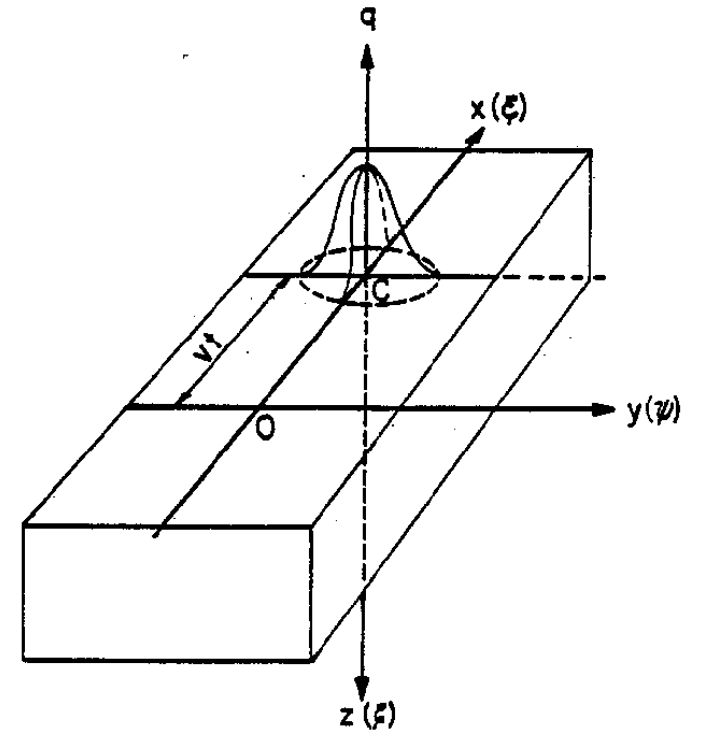
\includegraphics[width=0.50\linewidth]{../beamer-template/figures/eagar_tsai_og_figure.png}
          };
          \node[anchor=west,inner sep=0pt,text width=0.98\linewidth] at (0.0,3.05) {
            {\fontsize{15}{18}\selectfont
            \(\displaystyle
            \begin{aligned}
            T - T_0
            &= \frac{1}{2}\int_{0}^{t} dT_i \\
            &= \frac{q}{\pi\rho C_p\sqrt{4\pi\alpha}}
            \int_{0}^{t}
            \frac{(t-t')^{-1/2}}
                 {2\alpha(t-t')+\sigma^2} \\
            &\times
            \exp\Bigg[
            -\frac{(x-vt')^2+y^2}{4\alpha(t-t')+2\sigma^2}
            -\frac{z^2}{4\alpha(t-t')}
            \Bigg]\,dt'
            \end{aligned}
            \)
            }
          };
          \path (0,0) rectangle (1,4.25);
        \end{tikzpicture}
        \vfill
        {\fontsize{12.5}{15}\selectfont Eagar, T. W., \& Tsai, N. S. (1983). Temperature fields produced by traveling distributed heat sources. \textit{Welding Journal, 62}(12), 346--355.}
      \end{minipage}
    \end{column}
    \begin{column}{0.02\textwidth}
      \centering
      \vspace{-0.15em}
      \rule{0.5pt}{0.80\textheight}
    \end{column}
    \begin{column}{0.49\textwidth}
      \centering
      {\fontsize{22}{26}\selectfont\textcolor{sffblue}{\textbf{Refactored Eagar--Tsai Model}}\par}
      \vspace{0.18em}
      {\fontsize{15}{18}\selectfont Python library implementation with compiled-C speedup\par}
      \vspace{0.25em}

      \begin{tikzpicture}[x=\linewidth,y=1cm]
        \node[anchor=north,inner sep=0pt] at (0.37,-0.72) {
          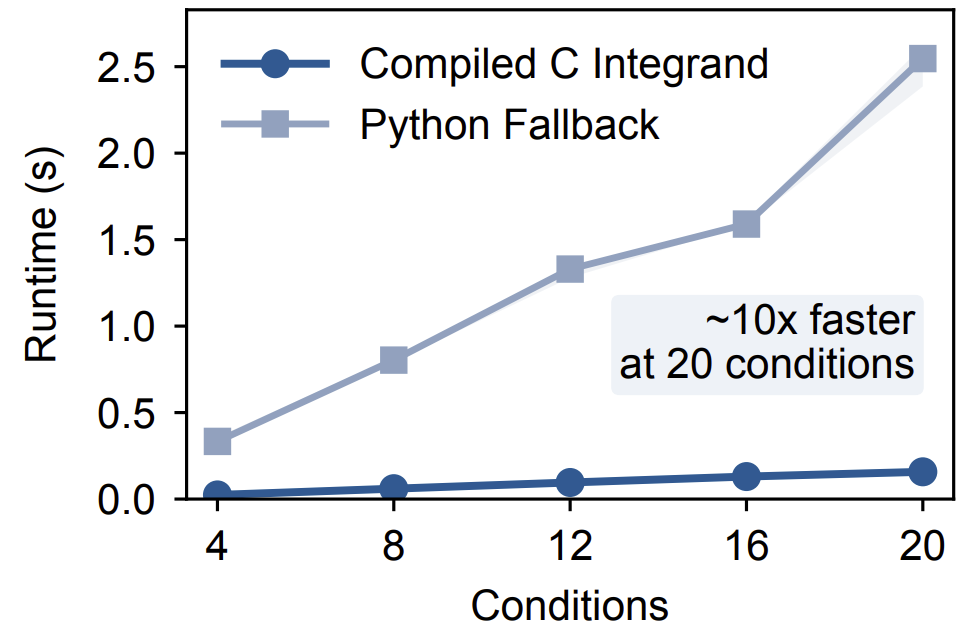
\includegraphics[width=0.66\linewidth]{../beamer-template/figures/dogu_figure_f.png}
        };
        \node[anchor=center,inner sep=0pt] at (0.82,-3.50) {
          
\includegraphics[width=0.23\linewidth]{../beamer-template/figures/logo.png}
        };
        \path (0,-4.45) rectangle (1,0);
      \end{tikzpicture}
      \vspace{0.05em}
      {\raggedright
      \begin{itemize}
        \item Uses the Rubenchik nondimensional integrand reformulation.
        \item Compiled C integrand removes Python overhead inside QUADPACK.
        \item Adds batch APIs, plotting, domain expansion, and field export.
      \end{itemize}
      }
    \end{column}
  \end{columns}
\end{frame}

\begin{frame}{Refractored ET Model}
  \begin{block}{Core idea}
    The refactored Eagar--Tsai workflow separates melt-pool prediction, 2D heatmap generation, and 3D temperature-field export into reusable steps.
  \end{block}
  \vspace{0.4em}
  \begin{itemize}
    \item Library-backed execution supports direct melt-pool evaluation from process and material inputs.
    \item Temperature fields can be exported as both dense CSV volumes and VTI files for downstream analysis.
    \item The workflow is structured for Bayesian correction, microstructure inference, and repeatable parameter studies.
  \end{itemize}
  \vspace{0.35em}
  {\fontsize{15}{18}\selectfont\textcolor{black!70}{Note to self: add speedup results and refer to Dogu's JOS paper.}}
\end{frame}

\begin{frame}{ET Thermal Cross Sections}
  \begin{columns}[T,onlytextwidth]
    \begin{column}{0.49\textwidth}
      \centering
      \begin{minipage}[t][0.68\textheight][c]{\linewidth}
        \centering
        
\includegraphics[width=\linewidth,height=0.68\textheight,keepaspectratio]{../beamer-template/figures/250_0.5/temperature_field_alloy0_250_0.5.png}
      \end{minipage}

      \vspace{0.25em}
      {\fontsize{15}{18}\selectfont Temperature heatmap for Hf$_2$Mo$_2$Ta$_{48}$W$_{48}$ (at.\%), $P = 250$ W and $V = 0.5$ m/s. Top: $z = 0$ surface. Bottom: $y = 0$ cross section.}
    \end{column}
    \begin{column}{0.49\textwidth}
      \centering
      \begin{minipage}[t][0.68\textheight][c]{\linewidth}
        \centering
        \includegraphics[width=\linewidth,height=0.68\textheight,keepaspectratio]{../beamer-template/figures/250_0.5/viewvti.png}
      \end{minipage}

      \vspace{0.25em}
      {\fontsize{15}{18}\selectfont 3D view of the ET melt pool for the same alloy and process condition.}
    \end{column}
  \end{columns}
\end{frame}

\begin{frame}{ET Thermal Gradient and Solidification Rate}
  \begin{columns}[T,onlytextwidth]
    \begin{column}{0.45\textwidth}
      \centering
      \begin{minipage}[t][0.58\textheight][c]{\linewidth}
        \centering
        
\includegraphics[width=\linewidth,height=0.58\textheight,keepaspectratio]{../beamer-template/figures/250_0.5/projected_GR_alloy0_250_0.5.png}
      \end{minipage}

      \vspace{0.25em}
      {\fontsize{15}{18}\selectfont Projection of $G$ and $R$ along the solidification front onto a $yz$ slice for Hf$_2$Mo$_2$Ta$_{48}$W$_{48}$ (at.\%), $P = 250$ W and $V = 0.5$ m/s.}
    \end{column}
    \begin{column}{0.08\textwidth}
      \centering
      \vspace{0.25\textheight}
      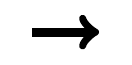
\begin{tikzpicture}
        \draw[->,line width=3.2pt,draw=black] (0,0) -- (0.85,0);
      \end{tikzpicture}
    \end{column}
    \begin{column}{0.45\textwidth}
      \centering
      \begin{minipage}[t][0.58\textheight][c]{\linewidth}
        \centering
        \includegraphics[width=\linewidth,height=0.58\textheight,keepaspectratio]{../beamer-template/figures/250_0.5/GR_map.png}
      \end{minipage}

      \vspace{0.25em}
      {\fontsize{15}{18}\selectfont GR Map calculated with Thermo-Calc CET Property Model for Hf$_2$Mo$_2$Ta$_{48}$W$_{48}$ (at.\%), $P = 250$ W and $V = 0.5$ m/s.}
    \end{column}
  \end{columns}
\end{frame}

\begin{frame}{ET Microstructure Classification}
  \begin{columns}[T,onlytextwidth]
    \begin{column}{0.49\textwidth}
      \centering
      \begin{minipage}[t][0.58\textheight][c]{\linewidth}
        \centering
        \includegraphics[width=\linewidth,height=0.58\textheight,keepaspectratio]{../beamer-template/figures/250_0.5/GR_map_overlay_alloy0_250_0.5.png}
      \end{minipage}

      \vspace{0.25em}
      {\fontsize{15}{18}\selectfont GR Map calculated with Thermo-Calc CET Property Model for Hf$_2$Mo$_2$Ta$_{48}$W$_{48}$ (at.\%), $P = 250$ W and $V = 0.5$ m/s.}
    \end{column}
    \begin{column}{0.49\textwidth}
      \centering
      \begin{minipage}[t][0.58\textheight][c]{\linewidth}
        \centering
        
\includegraphics[width=\linewidth,height=0.58\textheight,keepaspectratio]{../beamer-template/figures/250_0.5/projected_microstructure_alloy0_250_0.5.png}
      \end{minipage}

      \vspace{0.25em}
      {\fontsize{15}{18}\selectfont Projected microstructure classification along the solidification front onto a $yz$ slice for Hf$_2$Mo$_2$Ta$_{48}$W$_{48}$ (at.\%), $P = 250$ W and $V = 0.5$ m/s.}
    \end{column}
  \end{columns}
\end{frame}

\begin{frame}{Thermo-Calc AM Module}
\end{frame}

\begin{frame}{TCAM Thermal Cross Sections}
\end{frame}

\begin{frame}{TCAM Thermal Gradient and Solidification Rate}
\end{frame}

\begin{frame}{TCAM Microstructure Classification}
\end{frame}

\begin{frame}{Closing}
  \begin{block}{Takeaway}
    End with the decision, ask, or technical conclusion you want the audience to remember.
  \end{block}
  \vspace{0.5em}
  \begin{itemize}
    \item \deliverable{Deliverable}: Name the concrete output.
    \item \risk{Primary risk}: Name the hardest unresolved issue.
    \item \stage{Immediate next step}: Name the action that starts now.
  \end{itemize}
\end{frame}

\end{document}
